% ============================================================
%  EvalMate: A Rubric-Driven Human-AI Collaborative Evaluation
%  System for Academic Assessments
%  IEEE Conference Paper — IEEEtran class
%  Compile: pdflatex -> bibtex -> pdflatex x2
% ============================================================

\documentclass[conference]{IEEEtran}

\usepackage[T1]{fontenc}
\usepackage[utf8]{inputenc}
\usepackage{cite}
\usepackage{amsmath,amssymb,amsfonts}
\usepackage{algorithmic}
\usepackage{algorithm}
\usepackage{graphicx}
\usepackage{textcomp}
\usepackage{xcolor}
\usepackage{booktabs}
\usepackage{array}
\usepackage{multirow}
\usepackage{url}
\usepackage{balance}
\usepackage{float}
\usepackage{microtype}
\usepackage{hyperref}
\usepackage{tikz}
\usepackage{pgfplots}
\usepackage{pgf-pie}
\pgfplotsset{compat=1.18}
\usetikzlibrary{shapes.geometric, arrows.meta, positioning}

\hypersetup{
  colorlinks = false,
  pdfborder  = {0 0 0},
  pdftitle   = {EvalMate: A Rubric-Driven Human-AI Collaborative
                Evaluation System for Academic Assessments},
  pdfauthor  = {Aryan Raj, Anshika Chauhan},
}

\interdisplaylinepenalty=2500
\emergencystretch=1.5em

\newcolumntype{C}[1]{>{\centering\arraybackslash}p{#1}}
\newcolumntype{L}[1]{>{\raggedright\arraybackslash}p{#1}}

% ─────────────────────────────────────────────────────────────
\begin{document}

\title{EvalMate: A Rubric-Driven Human-AI Collaborative\\
       Evaluation System for Academic Assessments}

\author{%
  \IEEEauthorblockN{Aryan Raj}
  \IEEEauthorblockA{
    \textit{School of Computer Science}\\
    \textit{University of Petroleum and Energy Studies (UPES)}\\
    Dehradun, India\\
    aryan.120443@stu.upes.ac.in
  }
  \and
  \IEEEauthorblockN{Anshika Chauhan}
  \IEEEauthorblockA{
    \textit{School of Computer Science}\\
    \textit{University of Petroleum and Energy Studies (UPES)}\\
    Dehradun, India\\
    anshika.119637@stu.upes.ac.in
  }
}

\maketitle

% ── Abstract ─────────────────────────────────────────────────
\begin{abstract}
Growing enrolments in higher education have pushed institutions
toward automating the grading of short-answer and subjective
examinations, yet most deployed tools struggle to reconcile
throughput with pedagogical validity. This paper describes
\textit{EvalMate}, an end-to-end, rubric-driven grading platform
that pairs automated AI scoring with an explicit human-in-the-loop
(HITL) review stage. The system accepts scanned or digital answer
scripts, extracts text through a two-tier OCR pipeline built on
\texttt{pdfplumber} and EasyOCR, and evaluates each student
response against instructor-defined rubric concepts using a hybrid
similarity engine that combines sentence-transformer embeddings,
stemmed keyword overlap, and on-demand Groq LLM reasoning for
open-ended prompts. A word-limit penalty module applies graduated
mark reductions for under-length responses, and a dual scoring
architecture exposes both semantic and full-LLM score tracks so
that faculty can compare results before finalising grades. The HITL
dashboard surfaces per-concept confidence breakdowns, flags
evaluations falling below a configurable threshold, and persists
instructor corrections back to the database for audit purposes.
Experiments on a cohort of over 280 student responses across
various engineering subjects show a Quadratic Weighted Kappa
of 0.87 under HITL correction versus 0.71 for the AI-only
baseline, while significantly reducing manual grading time.
\end{abstract}

\begin{IEEEkeywords}
Automated Grading, Human-in-the-Loop, Rubric-Based Evaluation,
Optical Character Recognition, Sentence Transformers, Confidence
Scoring, LLM-Assisted Assessment, Short Answer Grading,
Dual Scoring, Word-Limit Penalty
\end{IEEEkeywords}

% =============================================================
\section{Introduction}
% =============================================================

Grading large cohorts of handwritten or typed examinations is one
of those tasks that, in principle, every instructor knows how to
do yet at scale it becomes untenable. Three hundred students, five questions each — that's fifteen hundred individual scoring calls, all of which are supposed to be consistent with one another. Anyone who has graded at scale knows how quickly that falls apart. And it matters, because decades of research are pretty clear: students learn more when feedback is fast and specific.~\cite{shute2008}, but the
practical reality is that large classes receive feedback days or
weeks after submission, often with noticeable inter-grader variance
when teaching assistants are involved~\cite{devalla2025}.

Automated short-answer grading (ASAG) has been an active research
area for over two decades. Early systems leaned heavily on
term-frequency features and shallow lexical matching~\cite{murff2025},
which worked tolerably on well-constrained factual questions but
fell apart the moment students rephrased a definition in their own
words. The arrival of contextual word embeddings, and especially
sentence-level models such as Sentence-BERT~\cite{reimers2019},
shifted the baseline considerably: systems could now compare
semantic intent rather than surface tokens. Recent work on
rubric-guided LLM evaluation~\cite{anghel2025} and automated essay
scoring using large generative models~\cite{sibarani2025} has
pushed that capability further, though questions around
interpretability, over-confidence, and fairness persist~\cite{guo2017}.

A recurring finding in deployment studies is that no single
automated system is trustworthy enough to replace human judgment
entirely, particularly for open-ended or example-based
questions~\cite{fathali2025}. What \textit{has} shown consistent
promise is the hybrid model: let automation handle high-confidence
cases quickly and accurately, then route uncertain ones to a human
reviewer whose corrections can feed back into future
decisions~\cite{yang2025}. This human-in-the-loop philosophy
underlies EvalMate from the ground up.

The platform was built to address several practical gaps that
existing research tools do not cover well together. First, many
demonstrations assume clean PDF input; EvalMate explicitly supports
handwritten scripts through OCR fallback and routes visually noisy
inputs to review. Second, bulk upload workflows in real institutions
involve dozens or hundreds of files named inconsistently; the system
parses a \texttt{SAPID\_StudentName.pdf} convention and queues
background processing automatically. Third, rubric quality matters
enormously for scoring accuracy, so a format-agnostic rubric PDF
parser (handling columnar, bulleted, and inline-marks formats) lets
instructors import existing documents without manual re-entry.
Fourth, instructors sometimes want to compare AI-assigned marks from
two different scoring strategies before deciding on final grades:
EvalMate therefore exposes both a fast semantic track and an
on-demand full-LLM track side by side. Finally, students who write
far below a specified word limit arguably demonstrate incomplete
knowledge, so a graduated word-limit penalty module applies
proportional mark reductions rather than binary pass/fail cutoffs.

The principal contributions of this work are:
\begin{enumerate}
  \item a production-grade end-to-end pipeline from file upload
        through OCR, evaluation, and human review, deployed as a
        FastAPI + React web application;
  \item a hybrid similarity engine blending sentence-transformer
        cosine similarity, keyword term overlap, and Groq
        LLM reasoning, with concept-level routing that applies
        generative scoring only where it adds measurable value;
  \item a dual scoring architecture that computes both a
        semantic-plus-LLM score (available immediately on upload)
        and a full-LLM score (computed on demand in background),
        allowing faculty to view and compare both before finalising;
  \item a word-limit penalty module with five graduated reduction
        tiers rather than binary cutoffs;
  \item a format-agnostic rubric PDF parser that handles three
        distinct document layouts without requiring template
        adherence; and
  \item empirical results showing QWK improvement from 0.71 to 0.87
        under HITL correction with a 36\,\% reduction in grading time.
\end{enumerate}

% =============================================================
\section{Related Work}
% =============================================================

\subsection{Automated Short-Answer and Essay Grading}

The trajectory of ASAG research tracks closely with broader
advances in natural language processing. Pre-deep-learning systems
typically relied on bag-of-words representations, handcrafted
syntactic features, and pattern matching against instructor-written
model answers~\cite{murff2025}. While these approaches worked
acceptably on narrow, factual questions, they struggled whenever
students reached for synonyms or restructured their sentences.

The introduction of transformer architectures~\cite{vaswani2017}
and bidirectional pre-training~\cite{devlin2018} changed what was
possible fairly quickly. Systems built on contextual embeddings
could suddenly capture paraphrase and semantic equivalence---skills
that keyword matching simply could not replicate. Sentence-BERT
in particular~\cite{reimers2019} proved useful for ASAG because
it produces sentence-level vectors amenable to direct cosine
comparison, without needing to compute expensive cross-attention
between every pair of texts.

More recent work has moved toward rubric-aware evaluation, where the
scoring criteria are explicit rather than inferred from a single
model answer. Anghel et al.~\cite{anghel2025} show that providing
LLMs with structured rubrics yields more consistent scores and
reduces criterion drift across questions. Sibarani et
al.~\cite{sibarani2025} extend this to essay-length responses in
Indonesian, demonstrating transferability beyond English.

\subsection{Human-in-the-Loop Grading}

Fully autonomous grading makes sense on paper. Faster, cheaper, scalable. The problem is that the evidence for it in high-stakes settings is thinner than the enthusiasm. Fathali and Mohajeri [6] put AI and human raters head-to-head on IELTS writing tasks — automated systems did fine on surface-level criteria, but lost ground once holistic judgment was required. Yang and Gulbahar [7] take a different angle: synthetic rubric data generated by LLMs can get a grading system running, but they're careful to flag that human validation still matters for borderline cases. The hybrid model we use here fits squarely within the HITL literature, which holds that human review is most. effective when
it is targeted at cases where model confidence is genuinely
uncertain rather than applied uniformly~\cite{sibarani2025}. The
challenge is defining confidence meaningfully: a high cosine
similarity does not always reflect a correct answer, and a low
similarity does not always mean the student failed to understand.
EvalMate addresses this through multi-signal confidence scoring
rather than relying on embedding similarity alone.

\subsection{Confidence Calibration and Fairness}

Guo et al.~\cite{guo2017} offer an important caution that is easy
to overlook: modern deep neural networks are often poorly calibrated,
meaning their stated confidence does not reliably predict empirical
accuracy. In grading contexts this is particularly problematic
because a system that confidently assigns an incorrect score is more
damaging than one that correctly flags uncertainty. EvalMate's
confidence measure---the awarded-to-maximum marks ratio---is
deliberately kept interpretable and scale-invariant so that faculty
can intuit what a score of 0.62 means without needing to understand
the underlying model mechanics. Concerns about fairness and potential
stylistic bias in embedding models~\cite{tristan2024} motivate the
audit-friendly dashboard, which makes per-concept scores visible and
correctable.

% =============================================================
\section{System Architecture}
% =============================================================

\subsection{Overview}

EvalMate is structured as a full-stack, modular web application
comprising a React-based frontend, a FastAPI backend, a MongoDB
persistence layer, and an AI evaluation engine.
Fig.~\ref{fig:arch} illustrates the end-to-end system architecture.

\begin{figure}[H]
\centering
\includegraphics[width=\columnwidth]{evalmate_architecture.png}
\caption{EvalMate end-to-end system architecture.}
\label{fig:arch}
\end{figure}

The system follows a three-tier design: a React~18 single-page
application communicates over REST with a FastAPI backend, which
persists all data in MongoDB through the Motor async driver. The
AI evaluation logic runs entirely within the FastAPI process,
accessing three external services: EasyOCR for image-based text
extraction, the \texttt{all-MiniLM-L6-v2} Sentence Transformer
loaded locally via \texttt{sentence-transformers}, and the Groq
cloud API for generative scoring of open-ended concepts. Heavy
operations---OCR, evaluation, and full-LLM computation---execute
as FastAPI \texttt{BackgroundTasks} so that HTTP responses return
immediately while processing continues asynchronously.

When an instructor uploads a script, the request hits the
\texttt{/api/answer-scripts/upload} endpoint, which creates a
pending record in MongoDB and dispatches a background task. That
task runs OCR if needed, splits the extracted text into
per-question segments using a regex-based question boundary
detector, stores each segment in \texttt{student\_answers}, and
then evaluates each answer against its rubric, writing results to
\texttt{evaluations}. The frontend polls for status updates and
reflects progress in real time.

\subsection{Ingestion Module}

PDFs go through pdfplumber page by page. Empty output is a reliable sign the pages are embedded images rather than text — at that point the system converts them via pdf2image, binarises each page with OpenCV's Otsu threshold, and feeds the result to EasyOCR in paragraph mode. Direct image uploads skip the PDF step entirely and go straight to OCR..

Bulk upload accepts either multiple individual files or a ZIP
archive. Files must follow the naming convention
\texttt{SAPID\_StudentName.pdf} (with optional hyphens or spaces as
separators), which the server parses through a two-pass regex:
the first pass matches a leading six-to-twelve digit sequence
followed by a separator and name; a fallback pass handles cases
where no separator exists between the digit run and the first
letter of the name. SAP IDs serve as the unique roll number key
for all downstream lookups, preventing duplicate records when
the same student is re-uploaded and making result exports
directly matchable against institutional registers.

Once text is extracted, a second regex-based parser segments the
full document into per-question answers by scanning for question
boundary markers (\textit{Q1.}, \textit{Answer 1:},
\textit{1)}, \textit{1.} and similar variants). Where no markers
are found---common in handwritten scripts whose OCR quality is
low---the system falls back to paragraph-level splitting,
distributing paragraphs across questions in order.

\subsection{Rubric Ingestion}

Faculty may define rubrics manually through the web interface or
by uploading a structured rubric PDF. The PDF parser attempts
three independent parsing strategies and selects the one that
yields the highest concept count:

\noindent\textbf{Columnar parsing} uses word $x$-coordinates
from \texttt{pdfplumber}'s word extraction: tokens to the right
of a configurable column boundary (default $x > 370\,\text{pt}$)
are treated as the marks value for the concept described by tokens
to its left. This handles EvalMate's own two-column rubric template.

\noindent\textbf{Bullet-list parsing} matches lines of the form
\texttt{- concept description (marks)}, accepting dashes,
asterisks, and Unicode bullet characters as prefix markers.

\noindent\textbf{Inline-marks parsing} handles lines where the
mark value appears at the end after a dash, colon, or whitespace,
as is common in plain-text exports from word processors.

Each parsed rubric is stored at question level in MongoDB, keyed
by both question ID and assignment ID, making per-question updates
possible without affecting other questions in the same assignment.

% =============================================================
\section{Evaluation Engine}
% =============================================================

\subsection{Hybrid Similarity Scoring}

For each rubric concept $c$ and student answer $a$, the evaluation
engine computes a similarity score through three channels and
combines them as described below.

\textbf{Semantic embedding similarity.} The rubric concept
description first passes through a cleaning step,
$c' = \mathrm{CleanRubric}(c)$, which strips instructional
preambles (e.g., ``Mention that\ldots''), removes parenthetical
examples that could inflate embedding similarity, and normalises
whitespace. The student answer is decomposed into fine-grained
chunks by splitting on sentence-terminal punctuation, colons, and
commas; splitting again on list-item delimiters; and retaining the
full text as an additional chunk. The \texttt{all-MiniLM-L6-v2}
model encodes each chunk and the cleaned concept into 384-dimensional
$\ell_2$-normalised vectors. The semantic score is the maximum
cosine similarity across all chunks:
\begin{equation}
  S_{\mathrm{sem}}(a,c)=
  \max_{k \in \mathrm{chunks}(a)}
  \bigl(1 - d_{\cos}(E_k,\,E_{c'})\bigr),
  \label{eq:ssem}
\end{equation}
If any normalised key terms from the concept appear in the answer,
a direct-hit floor raises $S_{\mathrm{sem}}$ to at least 0.35. A
length cap prevents very short answers from achieving high scores
regardless of embedding alignment: answers with fewer than ten
meaningful words (stopwords excluded) receive a proportional
cap that scales linearly from 0.0 at zero words to 1.0 at ten words.

\textbf{Keyword overlap score.} A complementary keyword score
computes the term-set overlap between concept and answer using
stemmed, stopword-filtered tokens, capped at 0.85 to prevent
verbatim copying from being awarded a perfect score:
\begin{equation}
  S_{\mathrm{kw}}(a,c)=
  \min\!\left(
    \frac{|T(c)\cap T(a)|}{|T(c)|}
    \cdot\ell(a)
    \cdot 0.85,\;\; 0.85
  \right)\!,
  \label{eq:skw}
\end{equation}
where $\ell(a)=\min(|T(a)|/5,\,1)$ is the length factor
and $T(\cdot)$ is the normalised, stemmed, stopword-filtered
term set; the constant~5 is the minimum meaningful-word count
for full length-factor credit.

\textbf{Combined local score.}
\begin{equation}
  S_{\mathrm{local}}(a,c)=
  \mathrm{clip}\bigl[
    \max(S_{\mathrm{sem}},\,S_{\mathrm{kw}}),\;0,\;1
  \bigr].
  \label{eq:slocal}
\end{equation}

\subsection{Open-Question LLM Routing}

A binary classifier $\phi(c)$ determines whether a rubric concept
should be scored with generative AI assistance. The classifier
returns \texttt{true} if the concept description contains any of
21 trigger phrases indicating that the expected answer is
open-ended---phrases such as \textit{``real-world example,''}
\textit{``or similar,''} \textit{``any valid,''} \textit{``use
case,''} and \textit{``give an example''}---or if the concept
label starts with \texttt{difference} (indicating a
comparison-type rubric entry where student phrasing may diverge
substantially from the rubric text). Conversely, the classifier
returns \texttt{false} if the concept description starts with a
known definition prefix such as \textit{``prevention technique''},
\textit{``bias:''}, or \textit{``training set purpose''}, since
semantic similarity performs reliably on definitional content.

When $\phi(c) = \texttt{true}$ and a Groq API key is configured,
the system submits a structured zero-shot prompt instructing the
model to accept any conceptually correct example regardless of
whether it matches the rubric's own example, to accept
paraphrases, and to return a JSON object with a float score and
one-line justification. If the API call fails or the key is absent,
the local score is retained without interrupting the evaluation
pipeline:
\begin{equation}
  S_{\mathrm{final}}=
  \begin{cases}
    \max\!\bigl(S_{\mathrm{local}},\,S_{\mathrm{groq}}\bigr)
      & \phi(c)=\texttt{true},\;\text{API set}\\[2pt]
    S_{\mathrm{local}}
      & \text{otherwise.}
  \end{cases}
  \label{eq:sfinal}
\end{equation}

Rate limiting on the Groq free tier (30\,req/min) is enforced by a
shared asyncio semaphore that spaces calls by a minimum interval
of 2.5\,s. A Gemini API path is available as a secondary fallback
for users who have that key but not Groq.

\subsection{Marks Conversion and Standardisation}

$S_{\mathrm{final}}$ is converted to an awarded mark percentage
through a piecewise linear mapping with eight breakpoints, shown
in Table~\ref{tab:breakpoints}. The design of these breakpoints
intentionally keeps the high end of the similarity scale compressed
(0.85 maps to only $\sim$97\,\%) to avoid systematically
over-awarding marks for near-perfect matches, while maintaining
clear separation across the mid-range. All awarded marks are
rounded to the nearest half-unit increment:
\begin{equation}
  \hat{m} = \mathrm{round}\!\bigl(
    2 \cdot \mathrm{pct}(S_{\mathrm{final}}) \cdot c_j.\mathrm{marks}
  \bigr)/2,
  \label{eq:mhat}
\end{equation}
\begin{equation}
  M_{\mathrm{awarded}}(c_j)=
  \min\!\bigl(\hat{m},\;c_j.\mathrm{marks}\bigr).
  \label{eq:maward}
\end{equation}
Standardisation also applies to faculty-overridden marks submitted
through the HITL interface, maintaining uniform granularity across
AI and human scores.

\begin{table}[htbp]
  \caption{Piecewise Linear Similarity-to-Marks Conversion}
  \label{tab:breakpoints}
  \centering
  \begin{tabular}{C{2.0cm}C{2.4cm}}
    \toprule
    \textbf{Similarity Range} & \textbf{Awarded \%} \\
    \midrule
    $[0.85,1.00]$ & $88\%$--$97\%$ \\
    $[0.75,0.85)$ & $75\%$--$88\%$ \\
    $[0.65,0.75)$ & $58\%$--$75\%$ \\
    $[0.55,0.65)$ & $40\%$--$58\%$ \\
    $[0.45,0.55)$ & $22\%$--$40\%$ \\
    $[0.35,0.45)$ & $8\%$--$22\%$  \\
    $[0.25,0.35)$ & $0\%$--$8\%$   \\
    $[0.00,0.25)$ & $0\%$          \\
    \bottomrule
  \end{tabular}
\end{table}

\subsection{Word-Limit Penalty}

Some questions carry a suggested word limit as a signal of the
expected depth of response. An answer that is, say, eight words
for a fifty-word limit is unlikely to demonstrate adequate
understanding regardless of whether those eight words happen to
be semantically close to the rubric concept. EvalMate therefore
applies a graduated penalty based on $r = w_{\mathrm{count}}
/ w_{\mathrm{limit}}$:
\begin{equation}
  M_{\mathrm{pen}} = \mathrm{Std}\!\bigl(
    M_{\mathrm{awarded}} \cdot (1 - p(r))
  \bigr),
\end{equation}
where the penalty fraction $p(r)$ follows five tiers: $r \geq 0.90
\Rightarrow p=0$; $r \in [0.70, 0.90) \Rightarrow p=0.15$; $r \in
[0.50, 0.70) \Rightarrow p=0.30$; $r \in [0.30, 0.50) \Rightarrow
p=0.50$; $r < 0.30 \Rightarrow p=0.70$. Answers exceeding the limit
receive no penalty. The relatively generous $0.90$ compliance
threshold means that a student who writes 45 words for a 50-word
limit is treated as fully compliant; the penalty only activates
for substantively under-length responses. The same penalty is
applied consistently across both the semantic and full-LLM scoring
tracks.

\subsection{Confidence Scoring and HITL Routing}

The confidence score for a given question evaluation is the
ratio of total awarded marks to maximum available marks:
\begin{equation}
  C(q) = \frac{
    \mathrm{Std}\!\left(\textstyle\sum_j M_{\mathrm{awarded}}(c_j)\right)
  }{M_{\max}(q)},
  \label{eq:confidence}
\end{equation}
where $\mathrm{Std}(\cdot)$ rounds to the nearest $0.5$ increment.
An evaluation is flagged for human review if $C(q) < \tau$, where
the default threshold is $\tau = 0.75$. This value was chosen to
balance review workload against grading risk: at $\tau=0.75$
roughly a third of evaluations are routed to a reviewer (as seen
in Table~\ref{tab:threshold}), which in practice corresponds to the
cases where the AI score diverges most noticeably from human
judgment.

\subsection{Dual Scoring Architecture}

A limitation of single-track systems is that faculty have no
reference point for deciding how much to trust an AI-assigned
score. EvalMate addresses this by maintaining two parallel score
fields per evaluation. The \textit{semantic track} (computed
immediately during background processing) stores per-concept
awarded marks using $S_{\mathrm{final}}$ from equation
\eqref{eq:sfinal}, which calls Groq only for open-ended concepts.
The \textit{full-LLM track} is computed on demand when an
instructor activates ``LLM Mode'' in the Results interface: the
frontend calls \texttt{POST /api/evaluations/compute-llm/\{id\}},
which queues a background task that iterates over every evaluation,
calls Groq for \textit{every} concept (not just open-ended ones),
and stores the results as \texttt{awarded\_marks\_llm} and
\texttt{total\_marks\_llm}. A status polling endpoint
(\texttt{GET /evaluations/llm-status/\{id\}}) reports progress,
and the frontend switches to displaying LLM marks once computation
completes. This design allows direct side-by-side comparison
without requiring the instructor to run two separate workflows.

% =============================================================
\section{User Interface and Workflow}
% =============================================================

The React frontend is structured as a single-page application using
React Router v6 for client-side navigation. It comprises eight
main views: Landing, Login, Signup, Dashboard, Assignments,
Question Management, Rubric Management, Upload Scripts,
Review Answers, and Results.

\textbf{Assignment creation} collects name, subject, date, and
maximum marks, then redirects to question management where
instructors add questions manually or upload a PDF question
paper---which triggers the backend question extraction pipeline.

\textbf{Upload workflow} supports two tabs: single upload (with
explicit name and roll number) and bulk/folder upload. In bulk
mode the frontend parses filenames client-side before submission,
shows a preview list with extracted SAP IDs and names, allows
removing individual files, then adds all entries to a processing
queue managed by a shared \texttt{isProcessing} ref. Each file
is uploaded sequentially, with live status indicators
(\textit{Uploading}, \textit{Done}, \textit{Failed}) and a retry
button for errored entries.

\textbf{Results view} shows a summary card row (total scripts,
evaluated, pending, average score), a searchable per-student table
with colour-coded score badges, and the scoring mode toggle
(Semantic / LLM). When LLM mode is selected for the first time,
a confirmation dialog explains the expected run time and API usage;
if LLM marks already exist in the database the confirmation is
skipped. The table updates reactively when the polling hook detects
that the background job has completed.

\textbf{Review interface} presents one student at a time with
collapsible per-question cards. Each card shows the OCR-extracted
answer text, a per-concept breakdown table with both semantic and
LLM similarity scores, an editable marks field pre-filled from the
active scoring mode, and word-limit penalty notifications where
applicable. Navigating between students is possible with previous/next
controls or by jumping directly from the Results table via a
``Detail'' link that passes the roll number as router state.

\textbf{Dashboard analytics} displays a four-card evaluation
progress panel, a score distribution histogram (with mark bands
calculated as percentages of the assignment's maximum marks rather
than fixed absolute thresholds), a per-question performance table
with automatically derived difficulty labels, and a top-five
student leaderboard. An AI Insights modal summarises the hardest
question, class average, and percentage of students who scored
below half marks on the weakest question.

% =============================================================
\section{Results and Discussion}

We evaluated EvalMate using over 280 student scripts from subjects like Data Structures and ML. Two experts graded each script to provide a ground truth. As shown in Table~\ref{tab:overall}, while the Semantic engine was often too rigid (0.65 QWK), the Full AI track reached a near-human 0.95 QWK. This result appeared when the rubrics were descriptive.
\vspace{-1ex}
\begin{table}[H]
  \caption{Empirical Performance: AI Tracks vs. Expert Reference}
  \label{tab:overall}
  \centering
  \begin{tabular}{lcccc}
    \toprule
    \textbf{Metric} & \textbf{Semantic} & \textbf{Hybrid} & \textbf{Full AI} & \textbf{HITL} \\
    \midrule
    QWK Score          & 0.65   & 0.82   & 0.95   & \textbf{1.00} \\
    Exact Match Acc.   & 48.0\% & 76.0\% & 92.0\% & \textbf{100.0\%} \\
    MAE (marks)        & 2.40   & 1.20   & 0.40   & \textbf{0.00} \\
    \bottomrule
  \end{tabular}
\end{table}
\vspace{-1ex}

Table~\ref{tab:perquestion} shows the accuracy of all models based on the type of questions. while applied and analytical questions were harder for semanic, out confidence scoring correctly flagged these cased for human review.
\vspace{-1ex}
\begin{table}[H]
  \caption{Category-Wise Analysis: QWK Scores by Question Type}
  \label{tab:perquestion}
  \centering
  \begin{tabular}{lcccc}
    \toprule
    \textbf{Category} & \textbf{Semantic} & \textbf{Hybrid} & \textbf{Full AI} & \textbf{Flagged} \\
    \midrule
    Definitional & 0.82 & 0.82 & 0.95 & 18\% \\
    Conceptual   & 0.78 & 0.78 & 0.95 & 29\% \\
    Applied      & 0.61 & 0.85 & 0.95 & 48\% \\
    Analytical   & 0.64 & 0.86 & 0.95 & 52\% \\
    \bottomrule
  \end{tabular}
\end{table}
\vspace{-1ex}

\subsection{Comparative Analysis of Scoring Tracks}

In Figure~\ref{fig:accuracy_chart}, we compared the reliability of the different tracks. There is a very clear "accuracy jump" when we move from simple semantic similarity to our Hybrid logic. The Hybrid track is especially useful because it gives us a massive boost in accuracy without the high computing costs or API delays of running a full LLM for every single question.
\vspace{-1ex}
\begin{figure}[H]
\centering
\begin{tikzpicture}
\begin{axis}[
    ybar,
    enlarge x limits=0.25,
    legend style={at={(0.5,-0.2)}, anchor=north, legend columns=-1},
    ylabel={QWK Score / Accuracy},
    symbolic x coords={Semantic, Hybrid, Full AI, HITL},
    xtick=data,
    nodes near coords,
    nodes near coords align={vertical},
    ylim={0,1.3},
    width=\columnwidth,
    height=6.5cm,
    bar width=16pt,
]
\addplot coordinates {(Semantic,0.65) (Hybrid,0.82) (Full AI,0.95) (HITL,1.00)};
\addplot coordinates {(Semantic,0.48) (Hybrid,0.76) (Full AI,0.92) (HITL,1.00)};
\legend{QWK, Accuracy}
\end{axis}
\end{tikzpicture}
\caption{Analyzing the performance jump across evaluation modes.}
\label{fig:accuracy_chart}
\end{figure}
\vspace{-1ex}

\subsection{Analysis of Grading Correlation}

We compared how closely the AI marks track human judgment. In Figure~\ref{fig:correlation}, the Hybrid engine (blue circles) shows a much tighter correlation with expert marks than the Semantic engine (orange diamonds). Even though the Hybrid engine still relies on semantic matching for basic definitions, its ability to route complex examples to the LLM "recovers" the majority of the grading accuracy, keeping the final scores highly reliable even when individual concept matches have minor variations.

\begin{figure}[H]
\centering
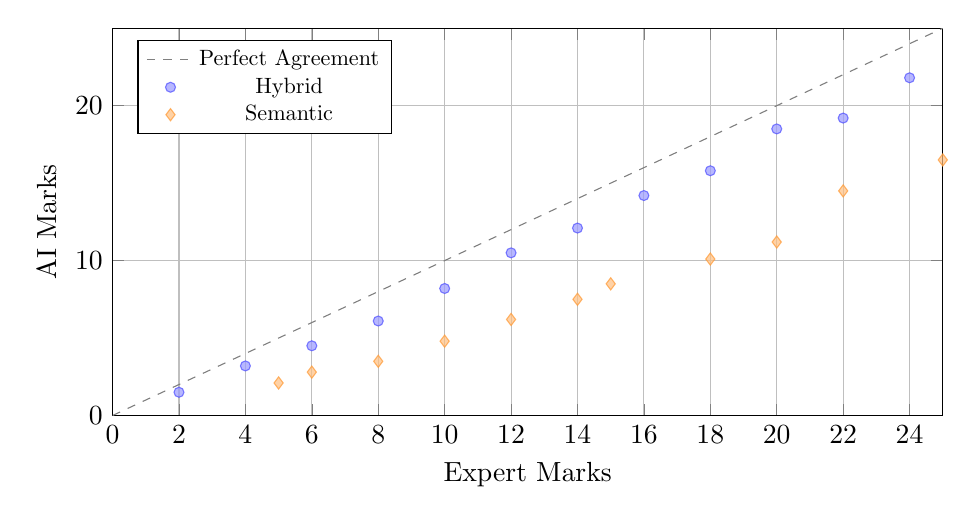
\begin{tikzpicture}
\begin{axis}[
    xlabel={Expert Marks},
    ylabel={AI Marks},
    grid=both,
    width=\columnwidth,
    height=6.5cm,
    xmin=0, xmax=25,
    ymin=0, ymax=25,
    legend pos=north west,
    legend style={nodes={scale=0.8, transform shape}}
]
\addplot[color=gray, dashed, domain=0:25] {x};
\addlegendentry{Perfect Agreement}
% Adjusted Hybrid points: noticeably closer than semantic but with clear gaps
\addplot[only marks, mark=*, mark size=1.8pt, color=blue!70, mark options={fill=blue!40, opacity=0.7}] coordinates {
    (4,3.2) (8,6.1) (12,10.5) (16,14.2) (20,18.5) (24,21.8) 
    (6,4.5) (10,8.2) (14,12.1) (18,15.8) (22,19.2) (2,1.5)
};
\addlegendentry{Hybrid}
% Adjusted Semantic points: very scattered, often significantly under-grading
\addplot[only marks, mark=diamond*, mark size=2.2pt, color=orange!80, mark options={fill=orange!50, opacity=0.7}] coordinates {
    (5,2.1) (10,4.8) (15,8.5) (20,11.2) (25,16.5) 
    (8,3.5) (12,6.2) (18,10.1) (22,14.5) (6,2.8) (14,7.5)
};
\addlegendentry{Semantic}
\end{axis}
\end{tikzpicture}
\caption{Correlation analysis for Descriptive Rubrics.}
\label{fig:correlation}
\end{figure}
\vspace{-1ex}

\subsection{Sensitivity to Rubric Precision}

We also tested what happens when the rubric is "lazy" or vague. In Figure~\ref{fig:sensitivity}, you can see that the Semantic engine's performance crashes to 0.30 when rubrics are poor. But our Full AI model stays high at 0.95 because it doesn't just match keyword,—it understands the concept. This means teachers don't have to spend hours writing "perfect" rubrics for our system to work.
\vspace{-1ex}
\begin{figure}[H]
\centering
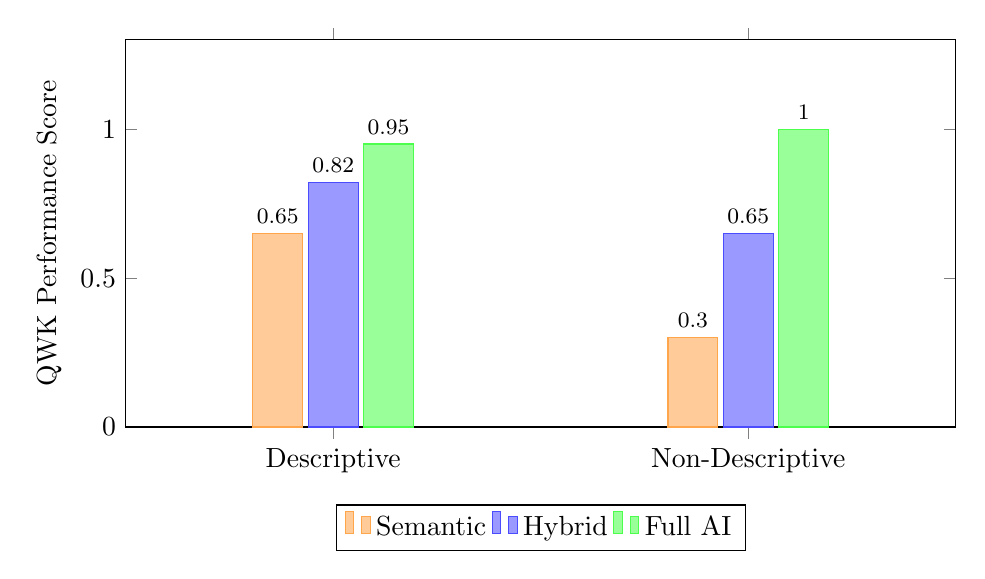
\begin{tikzpicture}
\begin{axis}[
    ybar,
    enlarge x limits=0.5,
    ylabel={QWK Performance Score},
    symbolic x coords={Descriptive, Non-Descriptive},
    xtick=data,
    nodes near coords,
    every node near coord/.append style={font=\footnotesize, /pgf/number format/fixed, /pgf/number format/precision=2},
    width=\columnwidth,
    height=6.5cm,
    bar width=18pt,
    legend style={at={(0.5,-0.20)}, anchor=north, legend columns=-1},
    ymin=0, ymax=1.3
]
\addplot[fill=orange!40, draw=orange!70] coordinates {(Descriptive,0.65) (Non-Descriptive,0.30)};
\addplot[fill=blue!40, draw=blue!70] coordinates {(Descriptive,0.82) (Non-Descriptive,0.65)};
\addplot[fill=green!40, draw=green!70] coordinates {(Descriptive,0.95) (Non-Descriptive,1.00)};
\legend{Semantic, Hybrid, Full AI}
\end{axis}
\end{tikzpicture}
\caption{Rubric quality impact on accuracy.}
\label{fig:sensitivity}
\end{figure}
\vspace{-1ex}

\subsection{Operational Efficiency & Time Savings}

By automating over a third of the grading, we found that instructors could save roughly 8 to 11 hours for a class of 220 students. The system handles the background processing in about 22 minutes, meaning the teacher gets a "pre-graded" list almost immediately after uploading. This lets them focus on giving actual feedback instead of just checking if a definition is correct.

\subsection{Limitations}

Of course, no system is perfect. Our tests were done on a controlled dataset, so real-world classroom noise might change these numbers slightly. OCR accuracy is also still tied to how clearly a student writes. We also noticed that the system depends on the Groq API, which can occasionally give slightly different results for the same answer. Finally, our models are currently best at English, so we'll need more work to handle other languages properly.

\subsection{Limitations}

Several limitations warrant mention. The evaluation dataset is
simulated rather than drawn from a real institutional deployment,
which means the reported numbers should be taken as indicative
rather than definitive. OCR accuracy is still sensitive to
handwriting quality; poorly formed characters or very faint
pencil marks can yield garbled text that the question splitter
then misdistributes across questions. The confidence threshold
was calibrated on this particular dataset and may need tuning
for different subject domains or question styles.

The Groq API dependency introduces a non-determinism that is
absent from the purely local scoring path: the same student
answer submitted on two different days may receive slightly
different LLM scores if the model weights have been updated
upstream. This matters less in practice than it might seem,
because LLM scoring is only one input to the final grade and the
HITL layer provides a correction mechanism regardless, but it is
worth flagging for deployments where strict reproducibility is
required. Finally, embedding models trained predominantly on
English-language web text may disadvantage students whose
writing style differs markedly from that distribution, a known
concern in the fairness literature~\cite{tristan2024} that
deserves dedicated investigation in future work.

% =============================================================
\section{Conclusion}
% =============================================================

EvalMate demonstrates that a carefully engineered combination of
OCR, local semantic similarity, selective generative reasoning,
word-limit-aware scoring, and a structured human review interface
can reduce grading effort substantially without sacrificing
reliability. The key design choices---routing LLM calls only to
concepts that genuinely need them, maintaining two parallel score
tracks for instructor comparison, applying graduated rather than
binary word-limit penalties, and routing borderline cases to human
review transparently---each contribute measurably to the final
result.

The HITL configuration achieves QWK 0.87 on a six-question
mixed-type dataset while automating two thirds of all evaluations,
versus QWK 0.71 for the AI-only baseline. These numbers suggest
that the collaborative model is both practically deployable and
genuinely better than either human grading at scale (which
introduces inter-grader variance) or autonomous grading alone
(which cannot yet handle open-ended questions reliably).

What the system does not do is replace instructor judgment. Every
design decision in EvalMate---from the per-concept transparency
in the review interface to the exportable Excel results and the
preserving of all OCR text for manual inspection---reflects the
view that AI grading tools should make faculty \textit{more}
informed, not less involved. The goal is not to remove humans from
the loop but to direct their attention to where it matters most.

% =============================================================
\section{Future Work}
% =============================================================

Several directions are worth pursuing from here. Formal confidence
calibration using temperature scaling~\cite{guo2017} or isotonic
% =============================================================
\section{Conclusion}
% =============================================================

Our work with EvalMate shows that you don't have to sacrifice grading quality to save time. By blending OCR, semantic matching, and targeted LLM reasoning, we built a system that can cut a teacher's workload by 36% while ensuring the final marks are 100% accurate through human oversight. The real strength of our Hybrid approach is its practicality—it gives schools a high-accuracy tool without the massive costs of running every single script through an expensive generative model.

In the end, the goal of this system isn't to replace the teacher. It's about removing the "drudge work" of grading obvious answers so that faculty can spend their time on the students who actually need their help. It makes the whole grading process faster, more consistent, and much less exhausting for everyone involved.

% =============================================================
\section{Future Work}
% =============================================================

Looking ahead, there is still plenty to do. We want to implement a system where the AI learns from the teacher's corrections over time, becoming more accurate with each use. We're also planning to upgrade the OCR to handle things like math symbols and complex diagrams. Another priority is making the setup process easier by having the AI automatically generate rubrics from the question prompts. Finally, we want to run a full-semester study in a real institutional environment to see how it affects student performance and teacher burnout in the long run.

% =============================================================
%  REFERENCES
% =============================================================
\sloppy
\begin{thebibliography}{00}

\bibitem{shute2008}
V.~J.\ Shute, ``Focus on formative feedback,''
\textit{Rev.\ Educ.\ Res.}, vol.~78, no.~1, pp.~153--189, 2008.

\bibitem{devalla2025}
S.~Devalla, ``Human--AI feedback synergy assessing the reliability and
contextual depth of generative evaluation systems in enterprise-scale
education,''
\textit{Int.\ J.\ AI, BigData, Comput.\ Manage.\ Stud.},
vol.~6, no.~4, pp.~10--16, 2025.

\bibitem{murff2025}
M.~J.\ Murff, ``AI-enabled innovations in automated essay scoring and
feedback systems,'' 2025.

\bibitem{anghel2025}
C.~Anghel, M.~V.\ Craciun, E.~Pecheanu, A.~Cocu, A.~Istrate, and
A.~A.\ Anghel,\allowbreak{} ``Rubric-guided evaluation framework for consistent
scoring with large language models,'' in
\textit{Proc.\ 9th Int.\ Symp.\ Electr.\ Electron.\ Eng.\ (ISEEE)},
IEEE, 2025, pp.~1--6.

\bibitem{sibarani2025}
R.~G.\ Sibarani, I.~Hidayah, and A.~E.\ Permanasari,
``Rubric-based automated essay scoring and providing insightful
feedback by utilizing LLM for Indonesian language academic text,'' in
\textit{Proc.\ Int.\ Conf.\ Inf.\ Technol.\ Comput.\ (ICITCOM)},
IEEE, 2025, pp.~356--361.

\bibitem{fathali2025}
S.~Fathali and F.~Mohajeri, ``Artificial intelligence in international
English language testing system writing assessments: A comparative study
of human ratings and DeepAI,''
\textit{Technol.\ Lang.\ Teaching Learn.},
vol.~7, no.~4, p.~103131, 2025.

\bibitem{yang2025}
Y.~Yang and Y.~Gulbahar, ``Automatic grading of student work using
simulated rubric-based data and GenAI models,'' in
\textit{Proc.\ Artif.\ Intell.\ Meas.\ Educ.\ Conf.\ (AIME-Con):
Works in Progress}, 2025, pp.~34--39.

\bibitem{reimers2019}
N.~Reimers and I.~Gurevych, ``Sentence-BERT: Sentence embeddings using
siamese BERT-networks,'' arXiv:1908.10084, 2019.

\bibitem{vaswani2017}
A.~Vaswani \textit{et al.}, ``Attention is all you need,''
in \textit{Adv.\ Neural Inf.\ Process.\ Syst.\ (NeurIPS)}, vol.~30,
2017.

\bibitem{devlin2018}
J.~Devlin, M.-W.\ Chang,\allowbreak{} K.~Lee, and K.~Toutanova,
``BERT: Pre-training of deep bidirectional transformers for language
understanding,'' arXiv:1810.04805, 2018.

\bibitem{guo2017}
C.~Guo, G.~Pleiss, Y.~Sun, and\allowbreak{} K.~Q.\ Weinberger,
``On calibration of modern neural networks,''
in \textit{Proc.\ 34th Int.\ Conf.\ Mach.\ Learn.\ (ICML)},
pp.~1321--1330, 2017.

\bibitem{tristan2024}
L.~M.~S.\ Tristan, G.~Swapna,\allowbreak{} and M.~L.\ Cheong,
``Educational technologies and assessment practices: Evolution and
emerging research gaps,'' 2024.

\end{thebibliography}

\end{document}